\documentclass[article]{jss}
\usepackage[utf8]{inputenc}

\providecommand{\tightlist}{%
  \setlength{\itemsep}{0pt}\setlength{\parskip}{0pt}}

\author{
Rolf Simoes, Gilberto Camara\\INPE, Brazil \And Victor Maus\\IIASA \And Alexandre Iwata\\IPEA, Brazil
}
\title{\pkg{SITS}: An R Package for Data Access, Visualisation, Filtering,
Clustering, Event Detection and Classification of Satellite Image Time
Series}

\Plainauthor{Rolf Simoes, Gilberto Camara, Victor Maus, Alexandre Iwata}
\Plaintitle{SITS: Satellite Image Time Series package}
\Shorttitle{SITS package}

\Abstract{
Using time series derived from big Earth Observation data sets is one of
the leading research trends in Land Use Science and Remote Sensing. One
of the more promising uses of satellite time series is its application
for classification of land use and land cover, since our growing demand
for natural resources has caused major environmental impacts. Given this
motivation, this package provides a set of tools for data access,
filtering, clustering and classification of satellite image time series.
}

\Keywords{satellite image time series, big Earth Observation data}

%% publication information
%% \Volume{50}
%% \Issue{9}
%% \Month{June}
%% \Year{2012}
%% \Submitdate{}
%% \Acceptdate{2012-06-04}

\Address{
      }

\usepackage{microtype} \usepackage{amsmath}

\begin{document}

\section{Introduction}\label{introduction}

Earth observation satellites provide a continuous and consistent set of
information about the Earth's land and oceans. Most space agencies have
adopted an open data policy, making unprecedented amounts of satellite
data available for research and operational use. This data deluge has
brought about a major challenge for Geoinformatics research:
\textit{How to design and build technologies that allow the Earth observation community to analyse big data sets?}

Since remote sensing satellites revisit the same place repeatedly, we
can calibrate their images so measures of the same place in different
times are comparable. These observation can be organised, so that each
measure from sensor is mapped into a three dimensional array in
space-time. From a data analysis perspective, researchers then have
access to satellite image time series (SITS). Using time series derived
from big Earth Observation data sets is one of the leading research
trends in Land Use Science and Remote Sensing.

A time-series of measurements of the same location in the surface of the
Earth can be considered as a historical record. When the images arise
for a dense record of frequent revisits, the temporal resolution of the
big data set is able to capture the most important land use changes.
Such dense time series allow researchers to which changes have taken
place in each location.

The benefits of remote sensing time series analysis arise when the
temporal resolution of the big data set is sufficient to capture the
most important changes. In this case, the temporal autocorrelation of
the data can be stronger than the spatial autocorrelation. In other
words, given data with adequate repeatability, a pixel will be more
related to its temporal neighbours rather its spatial ones. In this
case, \textit{time-first, space-later} methods will give better results
than the \textit{space-first, time-later} approach.

Time series of remote sensing data show that land cover changes do not
always occur in a progressive and gradual way, but they may also show
periods of rapid and abrupt change followed either by a quick recovery
\citep{Lambin2006}. Analyses of multiyear time series of land surface
attributes, their fine-scale spatial pattern, and their seasonal
evolution leads to a broader view of land-cover change. Satellite image
time series have already been applied to applications such as mapping
for detecting forest disturbance \citep{Kennedy2010}, ecology dynamics
\citep{Pasquarella2016}, agricultural intensification
\citep{Galford2008} and its impacts on deforestation \citep{Arvor2012}.

\section{Data Handling in SITS}\label{data-handling-in-sits}

The basic data unit in the sits package is the SITS tibble, which is

\begin{CodeChunk}

\begin{CodeInput}
> # Get a data set containing samples for two classes ("Cerrado" and "Pasture")
> cerrado.tb <- sits_getdata(file = system.file("extdata/samples/cerrado.json", package="sits"))
> cerrado.tb
\end{CodeInput}

\begin{CodeOutput}
# A tibble: 746 x 7
   longitude latitude start_date   end_date   label    coverage
       <dbl>    <dbl>     <date>     <date>   <chr>       <chr>
 1  -54.2313 -14.0482 2000-09-13 2001-08-29 Cerrado mod13q1_512
 2  -54.2313 -14.0482 2001-09-14 2002-08-29 Cerrado mod13q1_512
 3  -54.2313 -14.0482 2002-09-14 2003-08-29 Cerrado mod13q1_512
 4  -54.2313 -14.0482 2003-09-14 2004-08-28 Cerrado mod13q1_512
 5  -54.2313 -14.0482 2004-09-13 2005-08-29 Cerrado mod13q1_512
 6  -54.2313 -14.0482 2005-09-14 2006-08-29 Cerrado mod13q1_512
 7  -54.2313 -14.0482 2006-09-14 2007-08-29 Cerrado mod13q1_512
 8  -54.2313 -14.0482 2007-09-14 2008-08-28 Cerrado mod13q1_512
 9  -54.2313 -14.0482 2008-09-13 2009-08-29 Cerrado mod13q1_512
10  -54.2313 -14.0482 2009-09-14 2010-08-29 Cerrado mod13q1_512
# ... with 736 more rows, and 1 more variables: time_series <list>
\end{CodeOutput}
\end{CodeChunk}

this needs to be explained further\ldots{}.

\section{Using the Web Time Series Service
WTSS}\label{using-the-web-time-series-service-wtss}

To get a remote sensing time series, one first organises a large set of
EO data as a 3D array. From each pixel location in the array, one can
extract a time series of one or more variables for a temporal interval.
The WTSS service is independent of the actual data architecture used for
3D array store. It can work with solutions such as flat files, MapReduce
distributed datasets, array databases or object-relational databases. We
have implemented the service using both a set of flat files and the
SciDB array database management system \citep{Stonebraker2013}, with the
same external interface.

\begin{CodeChunk}

\begin{CodeInput}
> URL <- "http://www.dpi.inpe.br/tws/wtss"
> wtss_inpe <- sits_infoWTSS(URL)
\end{CodeInput}

\begin{CodeOutput}
-----------------------------------------------------------
The WTSS server URL is http://www.dpi.inpe.br/tws/wtss
Available coverages: 
itobi
merge
mixl8mod
mixl8mod_f
mod13q1_512
------------------------------------------------------------
\end{CodeOutput}
\end{CodeChunk}

\begin{CodeChunk}

\begin{CodeInput}
> # get information about a specific coverage
> sits_coverageWTSS(URL,"mod13q1_512")
\end{CodeInput}

\begin{CodeOutput}
----------------------------------------------------------------------------------
Coverage: mod13q1_512
Description: Vegetation Indices 16-Day L3 Global 250m
Source: https://lpdaac.usgs.gov/dataset_discovery/modis/modis_products_table/mod13q1
Bands: 
  name                            description
1 ndvi                      250m 16 days NDVI
2  evi                       250m 16 days EVI
3  red  250m 16 days red reflectance (Band 1)
4  nir  250m 16 days NIR reflectance (Band 2)
5 blue 250m 16 days blue reflectance (Band 3)
6  mir  250m 16 days MIR reflectance (Band 7)

Spatial extent: (-180, -90) - (180, 90)
Spatial resolution: (0.00208334, 0.00208334)
Projection CRS: +proj=longlat +ellps=WGS84 +datum=WGS84 +no_defs
Time range: 2000-02-18 to 2017-02-18
Temporal resolution: 16 days 
----------------------------------------------------------------------------------
\end{CodeOutput}

\begin{CodeInput}
> # choose a coverage
> coverage <- "mod13q1_512"
> # recover all bands
> bands <- c("ndvi", "evi", "nir")
> # a point in the transition forest pasture in Northern MT
> long <- -55.57320
> lat <- -11.50566
> # obtain a time series from the WTSS server for this point
> series.tb <- sits_getdata(longitude = long, latitude = lat, URL = URL, coverage = "mod13q1_512", bands = bands)
> # plot the series
> sits_plot (series.tb)
\end{CodeInput}


\begin{center}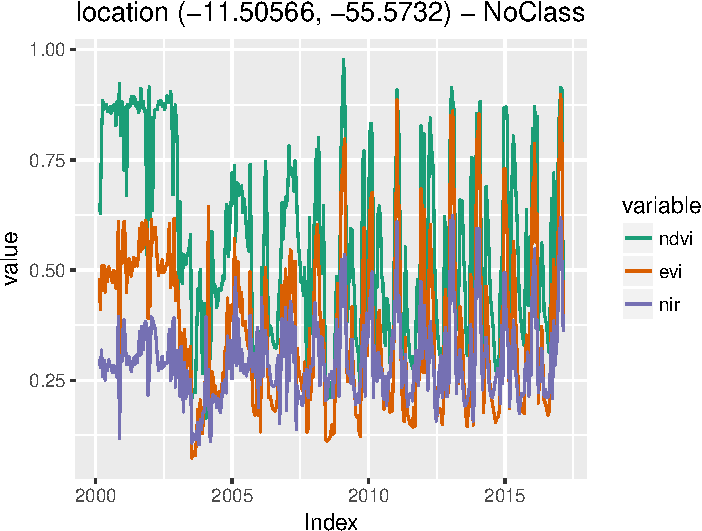
\includegraphics{sits_files/figure-latex/unnamed-chunk-7-1} \end{center}

\end{CodeChunk}

\section*{Acknowledgments}

This work is supported by the São Paulo State Foundation (FAPESP) under
grant 2014/08398-6 (``e-sensing: Big Earth observation data analytics
for land use and land cover change information''), and by the Germany
International Klimate Initiative under the RESTORE+
grant17\_III\_084\_Global\_A\_RESTORE+ (``RESTORE+: Addressing Landscape
Restoration on Degraded Land in Indonesia and Brazil''). Gilberto
Camara's work is also supported by CNPq (grant 312151/2014-4).

\bibliography{e-sensing.bib}


\end{document}

